Nuclear forensics comprises a large part of an investigation into a nuclear
incident, such as interdicted nuclear material or the detonation of a weapon
containing radioactive components.  The forensics portion of the investigation
encompasses both the analysis of nuclear material and/or related paraphernalia
as well as the interpretation of these results to establish nuclear material
provenance. The former has many technical aspects, relying on a range of
nuclear science and chemistry.  The latter involves intelligence and political
considerations of the material analyses for attribution. This review will only
consider the technical portion of the nuclear forensics workflow.

First discussed are the types of forensic investigations in Section
\ref{sec:types}, followed by an introduction to inverse problem theory in
Section \ref{sec:inverse} as a way to frame the forensics problem.

\subsection{Types of Nuclear Forensics Investigations}
\label{sec:types}

The technical programs researching improvements to the \acrshort{US}'s nuclear
forensics capabilities are split between the type of material being
investigated. The analysis of irradiated debris from a weapon has different
collection and measurement requirements than a mass of \gls{SNM}. This
separates the field into post-detonation and pre-detonation nuclear forensics.
While both are discussed below in Sections \ref{sec:postdet} and
\ref{sec:predet}, respectively, there is more focus on pre-detonation topics
since this work is based on \gls{SNF}. 

\subsubsection{Post-Detonation}
\label{sec:postdet}

Post-detonation nuclear forensics requires a diverse set of measurements to
obtain the following information: identification of nuclear material,
reconstruction of the weapon device design, and reactor parameters for nuclear
material provenance. This could apply to an improvised nuclear device or a
nuclear bomb.  In conjunction with the measurements and characterization are a
large array of logistical concerns, including recovery efforts, personnel
safety, and material collection cataloging and transportation.

In the case of a full explosion using fissile material, the collection of
materials and debris occurs as quickly as possible.  It can be in the crater
created by the explosion, further away from the center in the fallout, and in
the atmosphere above or downwind from the detonation. These are collected by
finding glass-like material near the epicenter, debris swipes in the fallout
region, and advanced particle collection in the atmosphere via an airplane,
respectively.  While the epicenter cannot be reached for some time, the debris
and atmosphere measurements of radioactive material can provide the yield of
the weapon and whether it was made using uranium or plutonium. This along with
other physical and chemical measurement allow device reconstruction to begin.
Attribution begins to narrow to specific countries or organizations based on
this information. \cite{aps_aaas_forensics}

The research needs for post-detonation focus on material collection and
analysis as well as nuclear device modeling for reconstruction purposes.
Ideally, most material sample collection would be done using automatic
instrumentation.  Additionally, bolstering the existing device modeling code
for reverse engineering is needed.  And, as with pre-detonation, a database of
standard materials must be both strengthened and centralized.
\cite{aps_aaas_forensics}

\subsubsection{Pre-Detonation}
\label{sec:predet}

Pre-detonation nuclear forensics investigations occur for every scenario in
which non-detonated nuclear material has been found or intercepted. Although
this could technically be an intact bomb, it is more likely that \gls{SNM}
intended for a weapon would be the target of an investigation since attempts at
materials smuggling are much more common.  The range of intact materials for
measurement could be as small as a gram-sized plutonium sample or as large as a
shipment of \gls{UOC}. The goal is to determine the provenance of the
\gls{SNM}, which in the case of \gls{SNF} is generally done by reconstructing
the irradiation process that created the material. 

For \gls{SNF}, where the material was obtained is the first step of the
investigation. This would be gleaned from the reactor parameters and storage
history (e.g., reactor type, cooling time, burnup), which requires first
measuring and calculating certain values: isotopic ratios, concentration of
chemical compounds, or existence of trace elements.  Both radiological methods
(e.g., gamma spectroscopy) and ionization methods (e.g., mass spectrometry)
measure these quantities.  

Although this is less of a humanitarian emergency than a post-detonation
investigation, it is still important to have rapid characterization
capabilities via on-site non-destructive analyses.  There could be weapons
construction already in progress that would need to be curtailed as quickly as
possible, or other related malicious intent that a faster investigation could
potentially derail.  As previously discussed in Section \ref{sec:motivation},
however, the faster measurements result in poor measurement quality. Also,
there is a need for research to combat the database issues, as an insufficient
forensics database can reduce the accuracy and/or certainty of a reconstructed
set of reactor parameters.  Another area of research is deeper study of known
forensics signatures or discovering new signatures with modeling, simulation,
or statistical methods. 

\subsection{Nuclear Forensics as an Inverse Problem}
\label{sec:inverse}

Nuclear forensics is a traditional inverse problem, which has been well
documented mathematically and applied to a range of scientific disciplines.
Understanding inverse problem theory can help systematically define the
limitations of certain solution methods.  This section provides an introduction
to the topic as well as its application to nuclear forensics. 

As outlined in a textbook on the formal approach to inverse problem theory
\cite{inverse_theory}, the study of a typical physical system encompasses three
areas:
\begin{enumerate}
  \itemsep-0.75em
  \item \textit{Model parameterization}
  \item \textit{Forward problem:} predict measurement values given model parameters
  \item \textit{Inverse problem:} predict model parameters given measurement values
\end{enumerate}

First, this shows that it is important to consider the parameters that comprise
a model; this is denoted as the \textit{model space}. This is not every
measurable quantity; domain knowledge is necessary to determine the model
space. In the nuclear forensics context for \gls{SNF}, this would consist of
the reactor operation history parameters. For example, this could be the time
since irradiation because the \gls{SNF} decays and material measurements are
different depending on when the measurement is taken.

Second, understanding the physical system also requires an understanding of the
forward problem. Predicting how a certain set of values of model parameters
will affect the resulting measurements is a problem with a unique solution.
The breadth of these end measurements provides the \textit{data space}, which
are all the conceivable results of a given forward problem. So for \gls{SNF}
this would be, e.g., the range of nuclide measurements typical of a commercial
reactor. 

Lastly, the inverse problem is predicting the model parameters (like time since
irradiation) given a solution (like an assay of nuclide measurements).  It is
statistical in nature; there is a probability that the measured nuclides are
caused by some value of a model parameter. Thus, the problem is
\textit{ill-posed} because a prediction is not guaranteed to be unique
\cite{skutnik_2016}. 

This can be done by directly inverting the model for a solution, or it can be
done from first principles or empirical relationships, which typically requires
iterative forward modeling that converges upon a solution. These two approaches
(direct inversion and forward modeling) are compared in some nuclear forensics
work in Reference \cite{inverse_compare}, where the authors are discussing the
discrimination capability of their approaches as it applies to plutonium powder
from reprocessing.  For forward modeling, they included two different linear
models to obtain the parameters of interest: a frequentist linear model and a
Bayesian linear model. For direct inversion, they employed principal components
regression and partial least squares regression. While the data set in the
paper did not provide enough measurements to effectively discriminate, it is
interesting to compare both inverse problem approaches in the same work. The
authors point out that finding agreement using several methods can be important
to proving the predictions are robust. 

Another example of iterative forward modeling being used in a nuclear forensics
context is in a suite of work using \gls{INDEPTH}, a tool developed at Oak
Ridge National Laboratory \cite{grogan_sensitivity1, grogan_sensitivity2,
grogan_indepth_2018, weber_2006, weber_2010, weber_2011}.  An initial report on
the methodology discusses the approach \gls{INDEPTH} uses \cite{weber_2006} and
a later report discusses \gls{INDEPTH} with more detailed examples
\cite{grogan_indepth_2018}.  

\begin{table}[!htb]
  \centering
  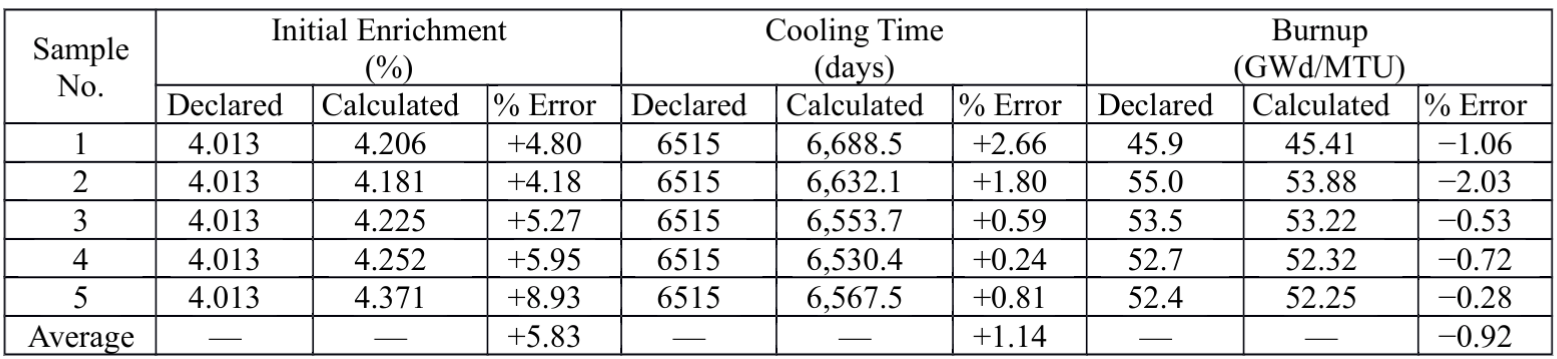
\includegraphics[width=\linewidth]{./chapters/litrev/indepth.png}
  \caption[Example of results from \acrshort{INDEPTH}]
          {Example set of results from \acrshort{INDEPTH} solving the inverse 
           problem being described in this work in Reference 
           \cite{grogan_indepth_2018}.}
  \label{tbl:indepth}
\end{table}

Through a nonlinear least-squares regression algorithm, repeated runs of
\gls{ORIGEN-ARP} are carried out given an initial guess. The squared error
residual is calculated from comparing the computed nuclide measurements against
a set of known nuclide measurements, and the repetition terminates when the sum
of the squared error is at some minimum.  \cite{weber_2006} This approach was
also tested with fission product measurements \cite{weber_2010} and later with
gamma spectra \cite{weber_2011}. Table \ref{tbl:indepth} shows an example of
the results from a set of samples that have the same \gls{U235} enrichment and
time since irradiation but different burnups.  The average error for the
enrichment is 5.83\%, but the other two parameters are both predicted within
approximately 1\% error. 

The iterative forward modeling approach has much merit, but another approach is
to use statistical methods to determine relationships between nuclide
measurements and reactor operation parameters. According to Reference
\cite{inverse_compare} in which forward modeling was compared against direct
inversion methods, the statistical approach in this work is also considered
direct inversion. The background for this is introduced next in Section
\ref{sec:mlback} and is later discussed within the context of nuclear forensics
in Section \ref{sec:stats4nf}.

\subsection{Nuclide Signatures for Nuclear Forensics of Spent Fuel}
\label{sec:nucs}

This work focuses on the nuclides created in the fuel (or pre-existing ones
that remain in the fuel) from its time in a nuclear reactor as the forensic
signatures of interest. Thus, what follows is a discussion on how some nuclides
can provide information about reactor type, burnup, \gls{U235} enrichment, and
time since irradiation.  Since the reactors considered here are common
commerial reactors that use uranium-oxide fuel, this configuration is the focus
and not, e.g., mixed-oxide fuel from reprocessing that could be used in a
\gls{LWR}.

The groups of nuclides tracked fall into two categories: actinides and fission
products. There are isotopes of both actinides and fission products tracked for
\gls{SNF} attribution in this work.  Few actinides are naturally occuring
(e.g., thorium and uranium), and the rest are created in the reactor core
through neutron captures of other actinides that do not lead to fission.
Fission products are the fragments of fissile isotopes (they can also be
created by neutron capture of the fragments, or radioactive decay of either of
these), which is usually \gls{U235}, but could be ${}^{239}\text{Pu}$ or
${}^{241}\text{Pu}$ (for uranium-oxide fuel).  The non-uranium and
non-plutonium actinides are present in much lower quantities than the fission
products.

In \gls{SNF}, the buildup of actinides is dependent on neutron capture (or the
lack thereof) of (initially) uranium isotopes and the buildup of fission
products is dependent on (mostly) \gls{U235} fissions. Thus, the neutron energy
spectrum in the reactor affects the levels of both actinides and fission
products.  This allows the distinguishing of different reactor types.  Their
creation is of course also linked to the initial enrichment and initial amounts
of various uranium isotopes via the number of fissions that can occur.  The
burnup of the fuel also impacts the amount of these nuclides, since more are
created as the fuel remains in the reactor core longer.  The radionuclides with
long half lives also can contribute to the time since irradiation
determination. While some nuclides might be a strong contributor to the
knowledge of one of the parameters, it is more common that they contribute
information about multiple. 

The buildup of ${}^{239}\text{Pu}$ is an example, where it is formed by the
neutron capture of ${}^{238}\text{U}$. This is dependent on the neutron energy,
so gives some indication of reactor type, but it is also dependent on the
amount of ${}^{238}\text{U}$ in the fuel, which gives some indication of
initial \gls{U235} enrichment. It also will capture neutrons and make higher
mass plutonium isotopes or fission the longer the fuel is in the reactor core.
Therefore, it is also linked to the burnup.

Two isotopes that 
